\section{How are we going to get there}

\subsection{Leading by example}

The principal technique throughout this book is leading by
example. What this means in this case is that the ideas are presented
primarily in terms of a coherent collection of examples, rendered as
\texttt{Scala} code, that work together to do something. Namely, these
examples function together to provide a prototypical web-based
application with a feature set that resonates with what application
developers are building today and contemplating building tomorrow.

Let's illustrate this in more detail by telling a story. We imagine a
cloud-based editor for a simple programming language, not unlike
\texttt{Mozilla}'s \texttt{bespin} . A user can register with the
service and then create an application project which allows them
\begin{itemize}
   \item to write code in a structured editor that understands the language;
   \item manage files in the application project;
   \item compile the application;
   \item run the application
\end{itemize}

\begin{figure}[tbp]
\begin{center}
{ \includegraphics[scale=.35]{/Users/lgm/work/src/projex/biosimilarity/trace/src/main/book/content/figures/RLambdaSignupPageScreenShot.pdf} }
\caption{ Example sign up page }
\end{center}
\end{figure}

% Thus, at broad strokes requests from the client app to the server break down into the following categories
% \begin{itemize}
%   \item edits to code
%   \item edits to project structure
%   \item compilation and execution requests
% \end{itemize}

These core capabilities wrap around our little toy programming
language in much the same way a modern IDE might wrap around
development in a more robust, full-featured language. Hence, we want
the capabilities of the application to be partially driven from the
specification of our toy language. For example, if we support some
syntax-highlighting, or syntax-validation on the client, we want that
to be driven from that language spec to the extent that changes to the
language spec ought to result in changes to the behavior of the
highlighting and validation. Thus, at the center of our application is
the specification of our toy language.

\begin{figure}[tbp]
\begin{center}
{ \includegraphics[scale=.35]{/Users/lgm/work/src/projex/biosimilarity/trace/src/main/book/content/figures/RLambdaREPLPageScreenShot.pdf} }
\caption{ Example REPL page }
\end{center}
\end{figure}

\begin{figure}[tbp]
\begin{center}
{ \includegraphics[scale=.35]{/Users/lgm/work/src/projex/biosimilarity/trace/src/main/book/content/figures/RLambdaSampleEvaluationResultPage.pdf} }
\caption{ Example evaluation result page }
\end{center}
\end{figure}

\subsubsection{Our toy language}

\paragraph{Abstract syntax}
%For our example we'll need a toy language.
Fittingly for a book about \texttt{Scala} we'll use the
$\lambda$-calculus as our toy language. \footnote{A word to the wise:
  even if you are an old hand at programming language semantics, even
  if you know the $\lambda$-calculus like the back of your hand, you
  are likely to be surprised by some of the things you see in the next
  few sections. Just to make sure that everyone gets a chance to look
  at the formalism as if it were brand new, a few recent theoretical
  developments have been thrown in. So, watch out!} The core
\textit{abstract} syntax of the lambda calculus is given by the
following \textit{EBNF} grammar.

\begin{mathpar}
  \inferrule* [lab=expression] {} {{M,N} ::=}
  \and
  \inferrule* [lab=mention] {} {x}
  \and
  \inferrule* [lab=abstraction] {} {\;| \; \lambda x . M}
  \and
  \inferrule* [lab=application] {} {\;| \; M N}
\end{mathpar} 

Informally, this is really a language of pure variable management. For
example, if the expression $M$ mentions $x$, then $\lambda x. M$ turns
$x$ into a variable in $M$ and provides a means to substitute values
into $M$, via application. Thus, $(\lambda x.M)N$ will result in a new
term, sometimes written $M[N/x]$, in which every occurrence of $x$ has
been replaced by an occurrence of $N$. Thus, $(\lambda x.x)M$ yields
$M$, illustrating the implementation in the $\lambda$-calculus of the
identity function. It turns out to be quite remarkable what you can do
with pure variable management.

\paragraph{A simple-minded representation}
At a syntactic level this has a direct representation as the following
\texttt{Scala} code.

\break
\begin{lstlisting}[language=Scala,mathescape=true]
  trait Expressions {
    type Nominal    
    // $M,N ::=$
    abstract class Expression

    // $x$
    case class Mention( reference : Nominal )
       extends Expression

    // $\lambda \; x_1,...,x_n.M$
    case class Abstraction(
       formals : List[Nominal],
       body : Expression
    )  extends Expression

    // $M N_1 ... N_n$
    case class Application(
       operation : Expression,
       actuals : List[Expression]
    )  extends Expression        
  }
\end{lstlisting}

In this representation each \emph{syntactic category}, EXPRESSION, MENTION,
ABSTRACTION and APPLICATION, is represented by a
\lstinline[language=Scala]!trait! or \lstinline[language=Scala]!case class!.
EXPRESSION's are \lstinline[language=Scala]!trait!'s because they
are pure placeholders. The other categories elaborate the syntactic
form, and the elaboration is matched by the
\lstinline[language=Scala]!case class!  structure. Thus, for example,
an ABSTRACTION is modeled by an instance of the
\lstinline[language=Scala]!case class! called
\lstinline[language=Scala]!Abstraction! having members
\lstinline[language=Scala]!formal! for the formal parameter of the
abstraction, and \lstinline[language=Scala]!body! for the
$\lambda$-term under the abstraction that might make use of the
parameter. Similarly, an APPLICATION is modeled by an instance of the
\lstinline[language=Scala]!case class! of the same name having members
\lstinline[language=Scala]!operation! for the expression that will be applied
to the actual parameter called (not surprisingly)
\lstinline[language=Scala]!actual!.

\paragraph{Currying}
The attentive reader will have noticed that there's a difference
between the abstract syntax and our \texttt{Scala} model. The abstract
syntax only supports a single formal parameter under
$\lambda$-abstraction, while the \texttt{Scala} model declares the
\lstinline[language=Scala,mathescape=true]!formals! to be of type
\lstinline[language=Scala,mathescape=true]!List[Nominal]!. The model
anticipates the encoding $\lambda \; x \; y . M \stackrel{def}{=}
\lambda \; x. \lambda \; y . M$. Given that abstractions are
first-class values, in the sense that they can be returned as values
and passed as parameters, this is a fairly intuitive encoding. It has
some pleasant knock-on effects. For example, when there is an arity
shortfall, i.e. the number of actual parameters is less than the
number of formal parameters, then it is both natural and useful simply
to return an abstraction. Thus, $(\lambda x y. f x y)u$ can be
evaluated to return $(\lambda y. f u y)$. This is an extremely
convenient mechanism to support partial evaluation.

\paragraph{Type parametrization and quotation}
One key aspect of this representation is that we acknowledge that the
abstract syntax is strangely silent on what the \emph{terminals}
are. It doesn't actually say what $x$'s are. Often implementations of
the $\lambda$-calculus will make some choice, such as
\lstinline[language=Scala]!String!s or
\lstinline[language=Scala]!Integers! or some other
representation. With \texttt{Scala}'s type parametrization we can
defer this choice. In fact, to foreshadow some of what's to come, we
illustrate that we never actually have to go outside of the basic
grammar definition to come up with a supply of identifiers.

In the code above we have deferred the choice of identifier. In the
code below we provide several different kinds of identifiers (the term
of art in this context is ``name''), but defer the notion of an
expression by the same trick used to defer the choice of identifiers.

\begin{lstlisting}[language=Scala]
  trait Nominals {
    type Term
    abstract class Name
    case class Transcription( expression : Term )
       extends Name
    case class StringLiteral( str : String )
       extends Name
    case class DeBruijn( outerIndex : Int, innerIndex : Int )
       extends Name
    case class URLLiteral( url : java.net.URL )
       extends Name
  }
\end{lstlisting}

Now we wire the two types together.

\begin{lstlisting}[language=Scala]
  trait ReflectiveGenerators
  extends Expressions with Nominals {
    type Nominal = Name
    type Term = Expression
  }
\end{lstlisting}

This allows us to use \emph{quoted} terms as variables in
$lambda$-terms! The idea is very rich as it begs the question of
whether such variables can be \emph{unquoted} and what that means for
evaluation. Thus, \texttt{Scala}'s type system is already leading
to some pretty interesting places! In fact, this is an instance of a
much deeper design principle lurking here, called two-level type
decomposition, that is enabled by type-level parametricity. We'll talk
more about this in upcoming chapters, but just want to put it on the
backlog.

\paragraph{Some syntactic sugar}
To this core let us add some syntactic sugar.

\begin{mathpar}
  \inferrule* [lab=previous] {} {{M,N} ::= ...}
  \and
  \inferrule* [lab=let] {} {\;| \; let \; x = M \; in \; N}
  \and
  \inferrule* [lab=seq] {} {\;| \; M;N}
\end{mathpar} 

This is sugar because we can reduce $let \; x \; = \; M \; in \; N$ to
$(\lambda x. N) M$ and $ M; N$ to $let \; x \; = \; M \; in \; N$ with
$x$ not occurring in $N$.

\paragraph{Digression: complexity management principle} In terms of
our implementation, the existence of this reduction means that we can
choose to have explicit representation of these syntactic categories
or not. This choice is one of a those design situations that's of
significant interest if our concern is complexity management. [Note:
brief discussion of the relevance of super combinators.]

\paragraph{Concrete syntax}
Now let's wrap this up in concrete syntax.

\begin{mathpar}
  \inferrule* [lab=expression] {} {{M,N} ::=}
  \and
  \inferrule* [lab=mention] {} {x}
  \and
  \inferrule* [lab=abstraction] {} {\;| \; \texttt{(} x_1 \texttt{,} ... \texttt{,} x_k \texttt{)} \; \texttt{=>} \; M}
  \and
  \inferrule* [lab=application] {} {\;| \; M\texttt{(} N_1 \texttt{,} ... \texttt{,} N_k \texttt{)}}
  \and
  \inferrule* [lab=let] {} {\;| \; \texttt{val} \; x \; \texttt{=} \; M \texttt{;} N}
  \and
  \inferrule* [lab=seq] {} {\;| \; M \texttt{;} N }
  \and
  \inferrule* [lab=group] {} {\;| \; \texttt{ \{ } M \texttt{ \} } }
\end{mathpar} 

It doesn't take much squinting to see that this looks a lot like a
subset of \texttt{Scala}, and that's because -- of course! --
functional languages like \texttt{Scala} all share a common core that
is essentially the $\lambda$-calculus. Once you familiarize yourself
with the $\lambda$-calculus as a kind of design pattern you'll see it
poking out everywhere: in \texttt{Clojure} and \texttt{OCaml} and
\texttt{F\#} and \texttt{Scala}. In fact, as we'll see later, just
about any DSL you design that needs a notion of variables could do
worse than simply to crib from this existing and well understood
design pattern.

If you've been following along so far, however, you will spot that
something is actually wrong with this grammar. We still don't have an
actual terminal! \emph{Concrete} syntax is what ``users'' type, so as
soon as we get to concrete syntax we can no longer defer our choices
about identifiers. Let's leave open the door for both ordinary
identifiers -- such as we see in \texttt{Scala} -- and our funny
quoted terms. This means we need to add the following productions to
our grammar.

\begin{mathpar}
  \inferrule* [lab=identifier] {} {{x,y} ::=}
  \and
  \inferrule* [lab=string-id] {} {\;| \; String}
  \and
  \inferrule* [lab=quotation] {} {\;| \; \texttt{@} \texttt{<} M \texttt{>}}
\end{mathpar} 

(The reason we use the \texttt{@} for quotation -- as will become
clear later -- is that when we have both quote and dequote, the former
functions a lot like asking for a \emph{pointer} to a term while the
latter is a lot like dereferencing the pointer.)

\paragraph{Translating concrete syntax to abstract syntax}
The translation from the concrete syntax to the abstract syntax is
compactly expressed as follows. Even if the form of the translation is
unfamiliar, it should still leave you with the impression that some
core of \texttt{Scala} is really the $\lambda$-calculus.

% \begin{mathpar}
%   \inferrule* {} {\meaningof{\lstinline[language=Scala,mathescape=true]!x!} = x}
%   \and
%   \inferrule* {} {\meaningof{\lstinline[language=Scala,mathescape=true]!(x) $\Rightarrow$! expr } = \lambda \; x . \meaningof{expr} }
%   \inferrule* {} {\meaningof{\lstinline[language=Scala,mathescape=true]!val x!} = let \; x = \meaningof{expr_1} in \meaningof{expr_2} }
% \end{mathpar}

\begin{lstlisting}[language=Scala,mathescape=true,frame=single,caption={translating concrete to abstract syntax},captionpos=b]
  $\ldb$ x $\rdb$ $=$ $x$
  $\ldb$ (x) => expr $\rdb$ $=$ $\lambda \; x . \ldb$ expr $\rdb$ 
  $\ldb$ expr( expr$_1$, ..., expr$_n$ ) $\rdb$
         $=$ $\ldb$ expr $\rdb$ $\ldb$ expr$_1$ $\rdb$ ... $\ldb$ expr$_n$ $\rdb$
  $\ldb$ val x = expr$_1$ ; expr$_2$ $\rdb$ $=$ $let$ $\ldb$ x $\rdb$ $=$ $\ldb$ expr$_1$ $\rdb$ $in$ $\ldb$ expr$_2$ $\rdb$
  $\ldb$ expr$_1$ ; expr$_2$ $\rdb$ $=$ $\ldb$ expr$_1$ $\rdb$ $;$ $\ldb$ expr$_2$ $\rdb$
  $\ldb$ { expr } $\rdb$ $=$ ( $\ldb$ expr $\rdb$ )
\end{lstlisting}

Further, the value of the explicit representation of sugar in terms of
structuring the translation should be clear. Of course, in a book
entitled \emph{Pro Scala} the best way to unpack this presentation
is in terms of a \texttt{Scala} implementation.

\begin{lstlisting}[language=Scala,mathescape=true]
  trait Compiler extends Expressions with Nominals {
    // Abstract away interning variables
    type Internist =
    {def intern( varExpr : Absyn.VariableExpr ) : Nominal}
    def internist() : Internist

    def intern( varExpr : Absyn.VariableExpr )
    : Nominal = { internist().intern( varExpr ) }
    def compileExpr( numericExpr : Absyn.Numeric )
    : Expression = {
      new IntegerExpression(
          numericExpr.integer_.asInstanceOf[Int]
      )
    }
    
    // $\ldb$ x $\rdb$ $=$ $x$
    def compileExpr( mentionExpr : Absyn.Mention )
    : Expression = {
      new Mention( intern( mentionExpr.variableexpr_ ) )
    }
    // $\ldb$ (x) => expr $\rdb$ $=$ $\lambda \; x . \ldb$ expr $\rdb$ 
    def compileExpr( abstractionExpr : Absyn.Abstraction )
    : Expression = {
      val fmls : List[Nominal] =
      abstractionExpr.listvariableexpr_.map(
      { ( vExpr : Absyn.VariableExpr ) => intern( vExpr )  }
      ).toList
      new Abstraction( fmls, compile( abstractionExpr.expression_ ) )	    
    }
    // $\ldb$ expr( expr$_1$, ..., expr$_n$ ) $\rdb$
    // $=$ $\ldb$ expr $\rdb$ $\ldb$ expr$_1$ $\rdb$ ... $\ldb$ expr$n$ $\rdb$
    def compileExpr( applicationExpr : Absyn.Application )
    : Expression = {
      new Application(
         compile( applicationExpr.expression_1 ),
         List( compile( applicationExpr.expression_2 ) )
      )
    }
    
    // $\ldb$ - $\rdb$ $:$ Mini-Scala => $\lambda$-calculus
    def compile( expr : Absyn.Expression )
    : Expression = {
      expr match {
        case value : Absyn.Value => {
          value.valueexpr_ match {
            case numericExpr : Absyn.Numeric =>
	    compileExpr( numericExpr )
          }
        }
        case numericExpr : Absyn.Numeric => {
          compileExpr( numericExpr )
        }
        case mentionExpr : Absyn.Mention => {
          compileExpr( mentionExpr )
        }
        case abstractionExpr : Absyn.Abstraction => {
          compileExpr( abstractionExpr )	    
        }
        case applicationExpr : Absyn.Application => {
          compileExpr( applicationExpr )
        }
      }
    }
    
    def parse( str : String ) : Absyn.Expression = {
      (new parser(
           new Yylex( new StringReader( str ) )
           ) ).pExpression()
    }
    
    def compile( str : String ) : Expression = {
      try {
        compile( parse( str ) )
      }
      catch {
        case e => { // log error 
          throw e
        }
      }
    }
  }
\end{lstlisting}

The first thing to notice about this translation is how faithfully it
follows the equational specification.

\paragraph{Structural equivalence and Relations or What makes abstract syntax abstract}

Apart from the fact that concrete syntax forces commitment to explicit
representation of terminals, you might be wondering if there are any
other differences between concrete and abstract syntax. It turns out
there are. One of the key properties of abstract syntax is that it
encodes a notion of equality of terms that is not generally
represented in concrete syntax.

It's easier to illustrate the idea in terms of our example. We know
that programs that differ only by a change of bound variable are
essentially the same. Concretely, the program
\lstinline[language=Scala]!( x ) => x + 5! is essentially the same as
the program \lstinline[language=Scala]!( y ) => y + 5!. By
``essentially the same'' we mean that in every evaluation context
where we might put the former if we substitute the latter we will get
the same answer. 

However, this sort of equivalence doesn't have to be all intertwined
with evaluation to be expressed. A little forethought shows we can
achieve some separation of concerns by separating out certain kinds of
\emph{structural} equivalences. Abstract syntax is where we express
structural equivalence (often written using $\equiv$, for example $M \equiv N$).
In terms of our example we can actually calculate when two
$\lambda$-terms differ only by a change of \emph{bound} variable,
where by bound variable we just mean a variable mention in a term also
using the variable as formal parameter of an abstraction.

Since we'll need that notion to express this structural equivalence,
let's write some code to clarify the idea, but because it will be more
convenient, let's calculate the variables not occurring bound,
i.e. the \emph{free} variables of a $\lambda$-term.

\begin{lstlisting}[language=Scala]
    def freeVariables( term : Expression ) : Set[Nominal] = {
      term match {
        case Mention( reference ) => Set( reference )
        case Abstraction( formals, body ) =>
	   freeVariables( body ) &~ formals.toSet
        case Application( operation, actuals ) =>
	   ( freeVariables( operation ) /: actuals )(
           { ( acc, elem ) => acc ++ freeVariables( elem ) } 
           )
      }
    }
\end{lstlisting}

In addition to this idea we'll need to represent exchanging bound
variables. A traditional way to approach this is in terms of
substituting a term (including variables) for a variable. A crucial
point is that we need to avoid unwanted variable capture. For example,
suppose we need to substitute $y$ for $x$ in a term of the form
$\lambda y.(x y)$. Doing so blindly will result in a term of the form
$\lambda y.(y y)$; but, now the first $y$ is bound by the abstraction
-- probably not what we want. To avoid this -- using structural
equivalence! -- we can move the bound variable ``out of the
way''. That is, we can first change the term to an equivalent one, say
$\lambda u.(x u)$. Now, we can make the substitution, resulting in
$\lambda u.(y u)$. This is what's called capture-avoiding
substitution. Central to this trick is the ability to come up with a
fresh variable, one that doesn't occur in a term. Obviously, any
implementation of this trick is going to depend implicitly on the
internal structure of names. Until we have such a structure in hand we
have to defer the implementation, but we mark it with a placeholder.

\begin{lstlisting}[language=Scala]
  def fresh( terms : List[Expression] ) : Nominal
\end{lstlisting}

Now we can write in \texttt{Scala} our definition of substitution.

\break
\begin{lstlisting}[language=Scala]
   def substitute(
   term : Expression,
   actuals : List[Expression], formals : List[Nominal]
  ) : Expression = {
    term match {
      case Mention( ref ) => {
	formals.indexOf( ref ) match {
	  case -1 => term
	  case i => actuals( i )
	}
      }
      case Abstraction( fmls, body ) => {
	val fmlsN = fmls.map(
	  {
	    ( fml ) => {
	      formals.indexOf( fml ) match {
		case -1 => fml
		case i => fresh( List( body ) )
	      }
	    }
	  }	      
	)
	val bodyN =
	  substitute(
	    body,
	    fmlsN.map( _ => Mention( _ ) ),
	    fmlsN
	  )
	Abstraction(
	  fmlsN,
	  substitute( bodyN, actuals, formals )
	)
      }
      case Application( op, actls ) => {
	Application(
	  substitute( op, actuals, formals ),
	  actls.map( _ => substitute( _, actuals, formals ) )
	)
      }
    }
  }
\end{lstlisting}

With this code in hand we have what we need to express the structural
equivalence of terms.

\begin{lstlisting}[language=Scala]  
  def `=a=`(
       term1 : Expression, term2 : Expression
   ) : Boolean = {
   ( term1, term2 ) match {
      case (
	Mention( ref1 ),
	Mention( ref2 )
      ) => {
	ref1 == ref2
      }
      case (
	Abstraction( fmls1, body1 ), Abstraction( fmls2, body2 )
      ) => {
	if ( fmls1.length == fmls2.length ) {
	  val freshFmls =
	    fmls1.map(
	      { ( fml ) => Mention( fresh( List( body1, body2 ) ) ) }
	    )
	  `=a=`(
	    substitute( body1, freshFmls, fmls1 ),
	    substitute( body2, freshFmls, fmls2 )
	  )
	}
	else false
      }      
      case (
	Application( op1, actls1 ),
	Application( op2, actls2 )
      ) => {
	( `=a=`( op1, op2 ) /: actls1.zip actls2 )(
	  { ( acc, actlPair ) =>
	    acc && `=a=`( actlPair._1, actlPair._2 )
	 }
	)
      }
    }
  }
\end{lstlisting}

This is actually some significant piece of machinery just to be able
to calculate what we mean when we write $M[N/x]$ and $M \equiv N$.
People have wondered if this sort of machinery could be reasonably
factored so that it could be mixed into a variety of variable-binding
capabilities. It turns out that this is possible and is at the root of
a whole family of language design proposals that began with Jamie
Gabbay's \texttt{FreshML}.

\paragraph{Digression: the internal structure of the type of variables}
If you've been paying attention, you will note that there's something
very funny going on in the calculation of
\lstinline[language=Scala]!freeVariables!. To actually perform the
\lstinline[language=Scala]!remove! or the
\lstinline[language=Scala]!union! we have to have equality defined on
variables. Now, this works fine for
\lstinline[language=Scala]!String!s, but what about
\lstinline[language=Scala]!Quotations!?

The question reveals something quite startling about the types\footnote{Note that here we mean the type of the entity in the model that represents variables -- not a typing for variables in the language we're modeling.} of
variables. Clearly, the type has to include a definition of
equality. Now, if we want to have an inexhaustible supply of
variables, then the definition of equality of variables must make use
of the ``internal'' structure of the variables. For example, checking
equality of \lstinline[language=Scala]!String!s means checking the
equality of the respective sequences of characters. There are a finite
set of characters out of which all \lstinline[language=Scala]!String!s
are built and so eventually the calculation of equality grounds
out. The same would be true if we used
\lstinline[language=Scala]!Integer!s as ``variables''. If our type of
variables didn't have some evident internal structure (like a
\lstinline[language=Scala]!String! has characters or an
\lstinline[language=Scala]!Integer! has arithmetic structure) and yet
it was to provide an endless supply of variables, then the equality
check could only be an \emph{infinite} table -- which wouldn't fit
inside a computer. So, the type of variables must also support some
internal structure, i.e. it must be a container type!

Fortunately, our \lstinline[language=Scala]!Quotation!s are
containers, by definition. However, they face another challenge: are
the \lstinline[language=Scala]!Quotation!s of two structurally
equivalent terms equal as variables? If they are then there is a
mutual recursion! Equivalence of terms depends on equality of
\lstinline[language=Scala]!Quotation!s which depends on equivalence of
terms. It turns out that we have cleverly arranged things so that this
recursion will bottom out. The key property of the structure of the
abstract syntax that makes this work is that there is an alternation:
quotation, term constructor, quotation, ... . Each recursive call will
lower the number of quotes, until we reach 0.

\paragraph{Evaluation -- aka operational semantics}

Here's the code

\begin{lstlisting}[language=Scala]
  trait Values {
    type Environment
    type Expression
    abstract class Value
    case class Closure(
       fn : List[Value] => Value
    ) extends Value
    case class Quantity( quantity : Int )
      extends Value
 }

 trait Reduction extends Expressions with Values {
   type Dereferencer = {def apply( m : Mention ) : Value }
   type Expansionist =
   {def extend(
     fmls : List[Mention],
     actls : List[Value]
     ) : Dereferencer}
   type Environment <: (Dereferencer with Expansionist)
   type Applicator = Expression => List[Value] => Value

   val initialApplicator : Applicator =
   { ( xpr : Expression ) => {
       ( actls : List[Value] ) => {
         xpr match {
           case IntegerExpression( i ) => Quantity( i )
           case _ => throw new Exception( "why are we here?" )
         }
       }
     }
   }
   
   def reduce(
      applicator : Applicator,
      environment : Environment
   ) : Expression => Value = { 
     case IntegerExpression( i ) => Quantity( i )
     case Mention( v ) => environment( Mention( v ) )
     case Abstraction( fmls, body ) =>
     Closure(
        { ( actuals : List[Value] ) => {
            val keys : List[Mention] =
 	    fmls.map( { ( fml : Nominal ) => Mention( fml ) });
            reduce(
	       applicator,
               environment.extend(
                  keys,
                  actuals ).asInstanceOf[Environment]
            )( body )
	  }
        }
     )
     case Application(
        operator : Expression,
        actuals : List[Expression]
     ) => {
	reduce( applicator, environment )( operator ) match {
	  case Closure( fn ) => {
	    fn.apply(
	      (actuals
	       map
	       {( actual : Expression) =>
		 (reduce( applicator, environment ))( actual )})
	    )
	  }
	  case _ =>
             throw new Exception( "attempt to apply non function" )
	}
      }
    case _ => throw new Exception( "not implemented, yet" )
  }
}
\end{lstlisting}

\subsubsection{What goes into a language definition}

Before moving to the next chapter it is important to digest what we've
done here. Since we've called out DSL-based design as a methodology
worthy of attention, what does our little foray into defining a
language tell us about language definition? It turns out that this is
really part of folk lore in the programming language semantics
community. At this point in time one of the commonly accepted
presentations of a language definition has three components:

\begin{itemize}
  \item syntax -- usually given in terms of some variant of BNF
  \item structural equivalence -- usually given in terms of a set of relations
  \item operational semantics -- usually given as a set of conditional
    rewrite rules, such as might be expressed in SOS format.
\end{itemize}

That's exactly what we see here. Our toy language can be completely
characterized by the following aforementioned half-page specification. 

\paragraph{Syntax}

\begin{mathpar}
  \inferrule* [lab=expression] {} {{M,N} ::=}
  \and
  \inferrule* [lab=mention] {} {x}
  \and
  \inferrule* [lab=abstraction] {} {\;| \; \lambda x . M}
  \and
  \inferrule* [lab=application] {} {\;| \; M N}
\end{mathpar} 

\paragraph{Structural equivalence}

\begin{mathpar}
  \inferrule*[left=$\alpha$-equivalence] { y \notin \mathcal{FN}( M ) } { \lambda x . M = \lambda y. M[y/x] }
\end{mathpar}

where

\begin{mathpar}
  \inferrule* {} {\mathcal{FN}( x ) = x} \and
  \inferrule* {} {\mathcal{FN}( \lambda x . M ) = \mathcal{FN}( M ) \backslash \{ x \} } \and
  \inferrule* {} {\mathcal{FN}( M N ) = \mathcal{FN}( M ) \cup \mathcal{FN}( N ) }
\end{mathpar}

and we write $M[y/x]$ to mean substitute a $y$ for every occurrence of $x$ in $M$.

\paragraph{Operational semantics}

\begin{mathpar}
  \inferrule*[left=$\beta$-reduction] {} {( \lambda x. M )N \to M[N/y] } \and
  \inferrule*[left=struct] { M \equiv M', M' \to N', N' \equiv N} {M \to N}
\end{mathpar}

\paragraph{Discussion}
This specification leaves open some questions regarding order or
evaluation. In this sense it's a kind of proto-specification. For
example, to get a left-most evaluation order you could add the rule

\begin{mathpar}
  \inferrule*[left=leftmost] { M \to M'} {M N \to M' N}
\end{mathpar}

The \texttt{Scala} code we wrote in the preceding sections is
essentially an elaboration of this specification. While this notation
is clearly more compact, it is not hard to recognize that the code
follows this structure very closely.

\subsection{Chapter map}

Taking a step back from the technical discussion let's recall what we
plan to cover and how we plan to cover it. Essentially, the book is
organized to follow the processing of \texttt{HTTP} requests from the
browser through the server and application code out to the store and
back.

\begin{itemize}
\item Chapter two introduces terminology, notation and concepts
  necessary for the rest of the book.
\item Chapter three looks at the organization of an \texttt{HTTP} server.
\item Chapter four investigates parsing the transport and application
  level requests.
\item Chapter five focuses on the application domain model.
\item Chapter six addresses at the navigation model.
\item Chapter seven reviews collections.
\item Chapter eight looks at the storage model.
\item Chapter nine investigates deployment of the application.
\item Chapter ten addresses new foundations for semantic query.
\end{itemize}

\begin{figure}[tbp]
\begin{center}
{ 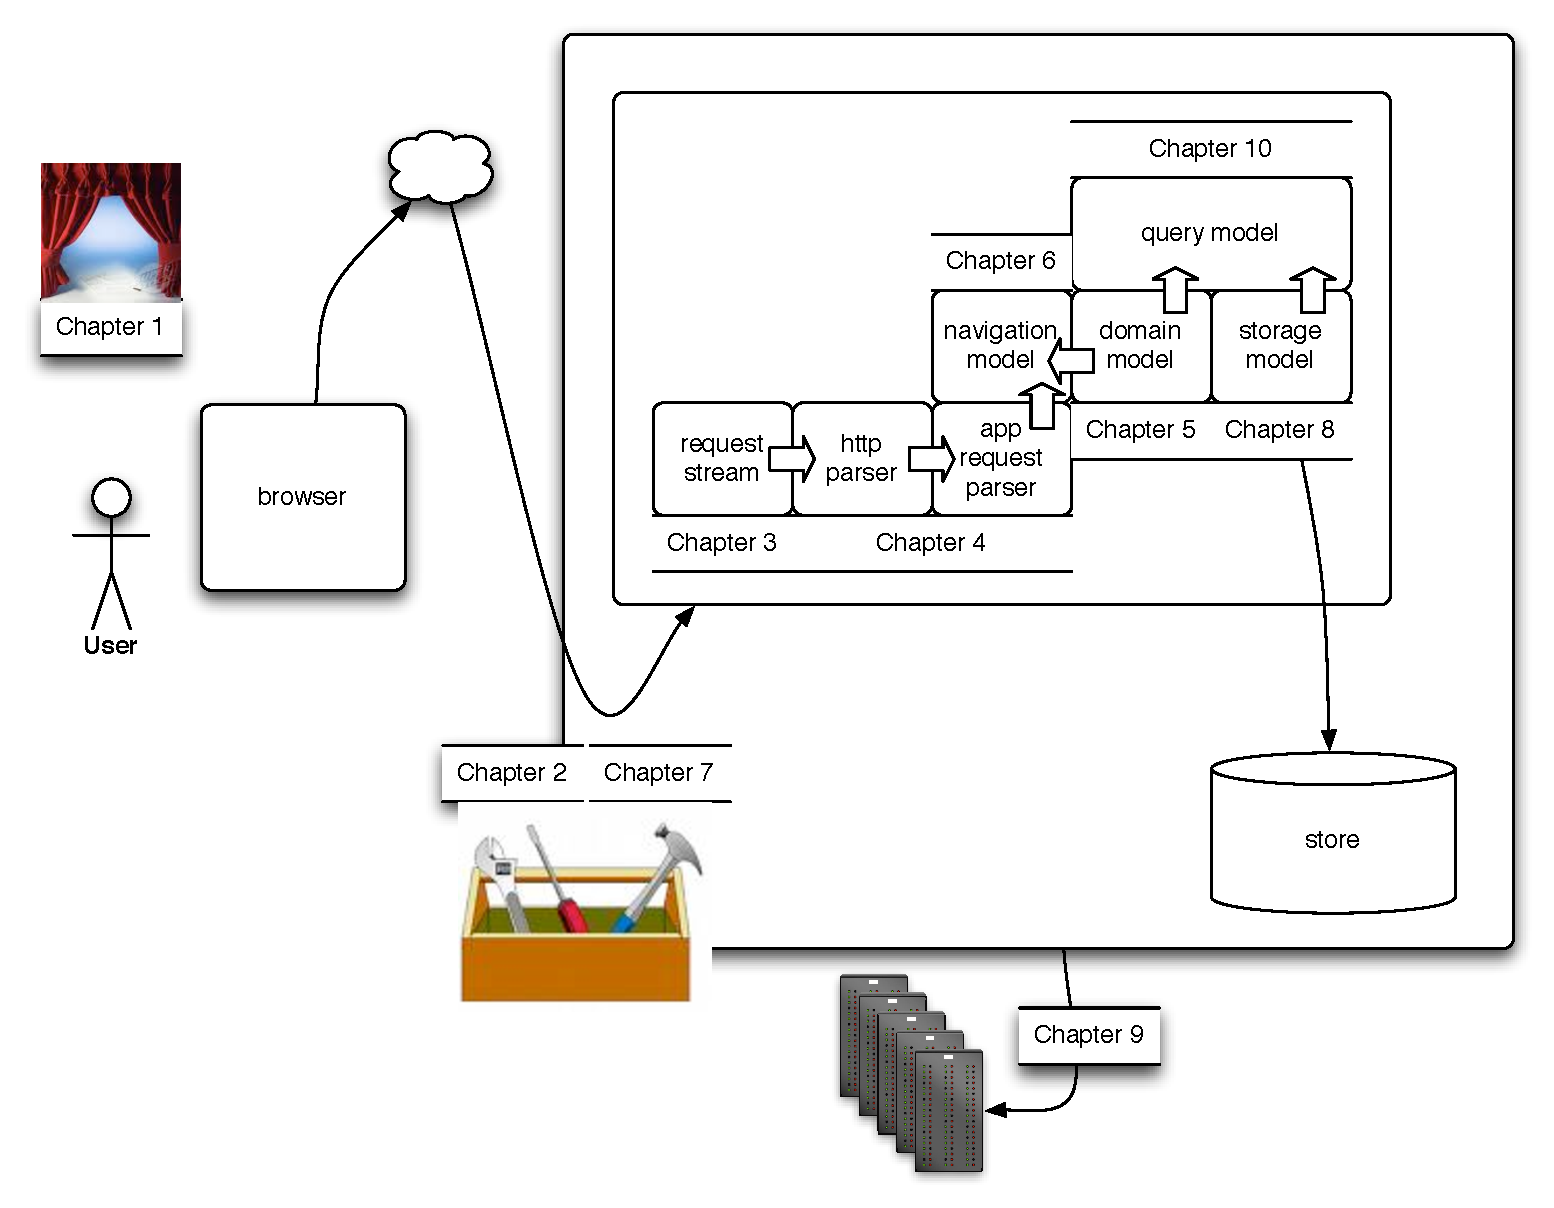
\includegraphics[scale=.65]{/Users/lgm/work/src/projex/biosimilarity/trace/src/main/book/content/figures/MonadicDesignPatternsChapterMap2.pdf} }
\caption{ Chapter map }
\end{center}
\end{figure}